\chapter{Methods}
\label{cha:methods}

This chapter describes the background of the developed Wrapper for integrating several drug related knowledge bases.
The project is called Semantic Drug Interface (SEDRI) and will be explained by the following sections in detail.

\section{Data integration}
\label{sec:data-integration}

Before the architecture and used data sets of SEDRI will be explained this section will discuss the different possibilities of integrating semantic data sets.

At first there is a distinction between virtual and local integration.
\todo{fundieren}
Virtual integration means that several federated data sets are queried and the results will be integrated virtually at query time independently of the source data sets.
In contrast, the local integration deploys an own copy of the data sets locally and integrates them based on certain criteria.
The main criteria that decides which approach is more suitable are query performance versus currentness of the data.

Virtual integration provides always up-to-date data because the knowledge bases are queried directly.
In the majority of cases this also leads to slower query times compared to local integration.
This is naturally caused by network times and the delay of the integration part.
Additionally it is not uncommon that knowledge bases are not available for a given time.
The local integration approach only queries one target and therefore is more performant in most of the cases.
The downside of this approach is that the data has to be updated regularly or the integration component will provide outdated data very quickly.
Example engines for the virtual integration of semantic knowledge bases are SPARQL 1.1 federated queries or tools like FedX that support also SPARQL <1.1.
With SPARQL 1.1 it is possible to query multiple tagets with one statement by using the \texttt{SERVICE} keyword.
Listing \ref{xx} gives an example of a federated query over two knowledge bases.
These federated queries are an easy yet powerful way to perform queries over multiple knowledge bases without the use of external tools.
The only problem is that the specific endpoints have to support SPARQL 1.1 which is not given in many cases.
An example of a local integration is the Linked Life Data project.
This project integrates multiple knowledge bases like Drugbank or Diseasome.
A disadvantage of the project is the policy that a full access including xx queries per hour requires a license payment.\todo{bedingungen detailieren}

\lstset{language=sparql}
\begin{lstlisting}[numbers=none,caption=Example of SPARQL 1.1 federated query]
  SELECT
\end{lstlisting}\todo{}
Which approach the SEDRI project uses will be explained in the following section.

\section{Architecture}
\label{sec:architecture}

As figure \ref{fig:arch_sedri} shows, the Semantic Drug Interface acts like an abstraction layer between the source data and the end user applications.
Besides the abstraction this layer can also be seen as integration layer.

\begin{figure}
  \centering
  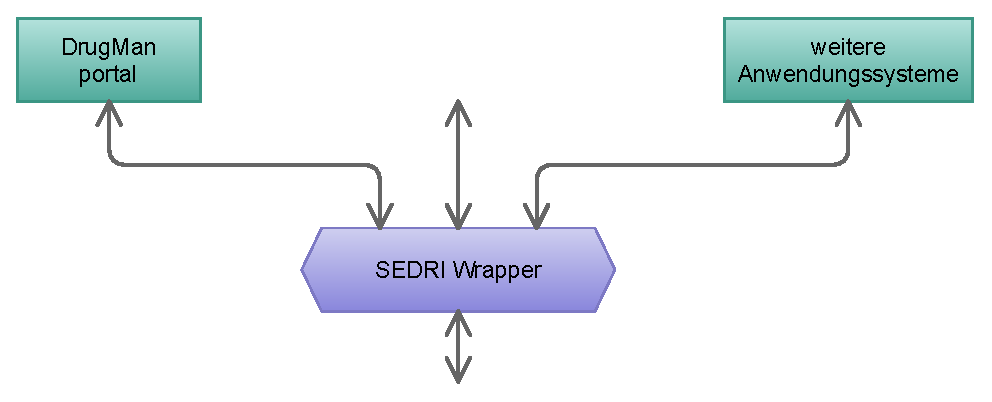
\includegraphics[scale=0.7]{methods/wrapper.eps}
  \caption{Overview of the architecture of SEDRI}
  \label{fig:arch_sedri}
\end{figure}
Section \ref{sec:data-integration} described the different possible approaches for integrating semantic knowledge bases.
SEDRI currently uses a virtual integration approach.
The reasons for this decision is the simplicity of the approach and the fact that possible applications expect always up-to-date knowledge.
Especially in the biomedical domain this is an important requirement.
SEDRI does not use the SPARQL 1.1 federated query possibility because many of the used data sets, or more specific the respectiv SPARQL endpoints, doesn't support this feature yet.
Therefore the different SPARQL endpoints are queried and the results merged.
The results are queried by a SPARQL \texttt{CONSTRUCT} statement.
This means that always full RDF resources are returned and not only single entities or literals.
These RDF resources can be returned by SEDRI in several representation formats, like \textit{Turtle}, \textit{RDF/XML} or \textit{JSON-LD}.
By default JSON-LD will be returned.
Other formats can be requested by setting the HTTP \texttt{Accept} Header to the appropriate MIME type.

To abstract from required background knowledge about the data sources, SEDRI predefines some API endpoints that are easily usable by only providing the necessary drug codes.
As such drug codes currently the ??? (ATC) code or the Drugbank ID are supported.
The API endpoints are designed to cover each phase of the WHO drug management life cycle.
The following list describes all available API endpoints that are provided by SEDRI and the respective queries and an example request.

\begin{itemize}
\item Drug-drug interactions -- \texttt{/ddi}:\\
This endpoint expects at least two drug codes and checks these drugs for drug-drug interactions.
In detail each possible combination of the given drugs is calculated and tested for interactions.
The maximum number of drug codes is unlimited.
This use case is mainly placed in the \textit{Selection} phase of the WHO drug management life cycle.
\begin{lstlisting}
  SELECT
\end{lstlisting}
\begin{lstlisting}
  GET http://sedri.de/ddi/?drug1=C07AB02&drug2=C07AB07&drug3=C01EB16
\end{lstlisting}

\item Side effects -- \texttt{/sideeffects}:\\
The side effects endpoint expects one drug code and returns all available side effects of this drug.
This component supports primarily the phase \textit{Use}.
\begin{lstlisting}
  SELECT
\end{lstlisting}
\begin{lstlisting}
  GET http://sedri.de/sideeffects/?drug=C07AB02
\end{lstlisting}

\item Procurement -- \texttt{/procure}:\\
The procurement component returns the possible manufacturers and packagers for a given drug code.
Trivialy this component supports the procurement phase of the drug management life cycle.

\begin{lstlisting}
  SELECT
\end{lstlisting}
\begin{lstlisting}
  GET http://sedri.de/procure/?drug=C07AB02
\end{lstlisting}

\item Drug proposals -- \texttt{/proposals}:\\
This endpoint proposes several drugs to a given disease.
To specify the disease currently only the Medical Subject Headings (MeSH) ID is supported.
As results the respective URIs to the drugs are returned.
With these URIs more details can be retrieved.
This component covers the \textit{Selection} phase.
\begin{lstlisting}
  SELECT
\end{lstlisting}
\begin{lstlisting}
  GET http://sedri.de/proposal/?code=D006973
\end{lstlisting}

\item Pharmacogenetics meta data -- \texttt{/details}:\\
This component returns several meta data to a given drug code.
The results contains mainly pharmacogenetic information like dosages, the affected organism or the route of elimination.
In the WHO drug management life cycle this component covers the mainly the \textit{Use} phase but also in parts the \textit{Selection} phase.

\begin{lstlisting}
  SELECT
\end{lstlisting}
\begin{lstlisting}
  GET http://sedri.de/details/?drug=C07AB02
\end{lstlisting}

\end{itemize}

\section{Data sets}
\label{sec:data-sets}

% \begin{itemize}
% \item übersicht datensätze
%   \begin{itemize}
%   \item tabellarisch/grafisch
%   \item proprietäre quellen die nicht verwendet werden konnten
%     \begin{itemize}
%     \item senger et al
%     \end{itemize}
%   \end{itemize}
% \end{itemize}

\begin{tabular}{p{\textwidth/5}|p{\textwidth/3}|p{\textwidth/3}}
  Data set & Description & Usage\\
  \hline
  DBpedia & DBpedia provides data that is received by multiple Wikipedia and therefore includes many cross domain information. & The data set is used for converting the given ATC codes of drugs to Drugbank IDs for a better processing. The second use case is the proposal endpoint where DBpedia is used for the assignment of the Diseasome URI to a given MeSH code. \\
  Drugbank & Drugbank is a large knowledge base that contains many different information about drugs and their meta data such as interactions, dosages or manufacturers. & Drugbank is the main knowledge base used by SEDRI. It provides information for nearly each given endpoint, except the side effects.\\
  SIDER & The main domain of SIDER are side effects of drugs. Besides this it provides not much additional information. & side effects\\
  Drug Interaction Knowledge Base & B & interactions \\
  PharmGkb & B & side effects\\
  Diseasome & B & drug proposals
\end{tabular}

%%% Local Variables: 
%%% mode: latex
%%% TeX-master: "../thesis"
%%% End: 
